

\chapter{SIMD MOAB Bounding Volume Hierarchy}\label{ch:simd_bvh}


\section{Introduction}

As established in Section \ref{sec:problem-statement}, the dominant source of
additional runtime in DAGMC is spent in the ray tracing process used to satisfy
the Monte Carlo geometry queries outlined in Section \ref{sec:mc-geom-queries}.
The focus of the work in this chapter is improvements on the performance of the
ray tracing process through the application of SIMD-oriented programming in the
bounding volume hierarchies used in DAGMC. Some preliminary work was performed
in this area by replacing the ray tracing kernel used in DAGMC (MOAB's oriented
bounding box tree) with a kernel produced by Intel, called Embree.

\section{Linking DAGMC with Intel's Embree}\label{sec:embree}

Embree is the result of a an effort to produce a performant CPU-based raytracer
as a demonstration of the expanding capabilities of modern CPU architectures
\cite{Wald_2014}. In both construction and traversal of BVHs, Embree takes
advantage of many of the latest developments in BVH research by using modern
chipset architecture capabilities via vectorization at an implementation level
as described in Section \ref{subsec:arch} of this work. The combination of these
effects leads to a very powerful raytracing tool in terms of performance, as
demonstrated by the many projects which have incorporated Embree as their
production ray tracing kernel such as Corona, Autodesk, FluidRay, and
Brighter3D.As a result of its success in other areas, Embree was selected to be
applied in DAGMC to satisfy geometric queries for MCNP. The resulting
combination of these tools will be reffered to as EmDAG.

\subsection{Transferring DAGMC Model's to Embree Scenes}%%Status:Done%%

The process of employing Embree as DAGMC's ray tracer begins by establishing an
equivalent representation of the MOAB mesh in Embree. In comparison to MOAB,
Embree is limited in its ability to represent the underlying topological
structure of a model. This topology is necessary and used advantageously during
particle tracking in DAGMC by reducing the set of triangles queried to those of
the particle's current volume and thus reducing the number of point containment
queries. However, a method was discovered to represent enough of the topology to
meet the requirements of DAGMC transport. The highest level representation in
Embree is referred to as a scene. Each scene may contain one or more geometries
or triangle surface meshes. Fortunately, this system is enough to create a
workable representation of DAGMC meshes in which MOAB volumes are the equivalent
of Embree scenes and MOAB surfaces are represented in their respective scenes as
surfaces. This method provides a one-to-one mapping of MOAB volumes and surfaces
to their corresponding entities in Embree and allows all topology-based
operations to proceed inside of DAGMC in their usual manner. In this way, the
requirement for topological information in DAGMC at the surface and volume level
is met. Next, transfer of the primitive mesh data is considered.

Scenes do not share mesh data as volumes are able to do in MOAB, so the triangle
connectivity of each surface is reproduced in each scene they belong
to. Fortunately, Embree does allow the sharing of vertices between scenes. In
order to take advantage of this feature, all of the vertices in the MOAB mesh
are provided in the Embree instance as a global vertex buffer. Surfaces from all
scenes can then be defined by a connectivity of vertices from this global pool
of points. This method guarantees that the each surface can be represented by
the same set of stored vertices in each scene it belongs to giving the exact
same representation in each scene. It greatly simplifies particle tracking by
guaranteeing that the same surfaces will not overlap each other in the different
scenes they are a part of by doing the conversion of points from the MOAB
database to Embree only once. Additionally, this method will maintain
watertightnes at the boundaries between surfaces ensuring the same model
fidelity as the representation in MOAB.

\begin{figure}
  \centering
  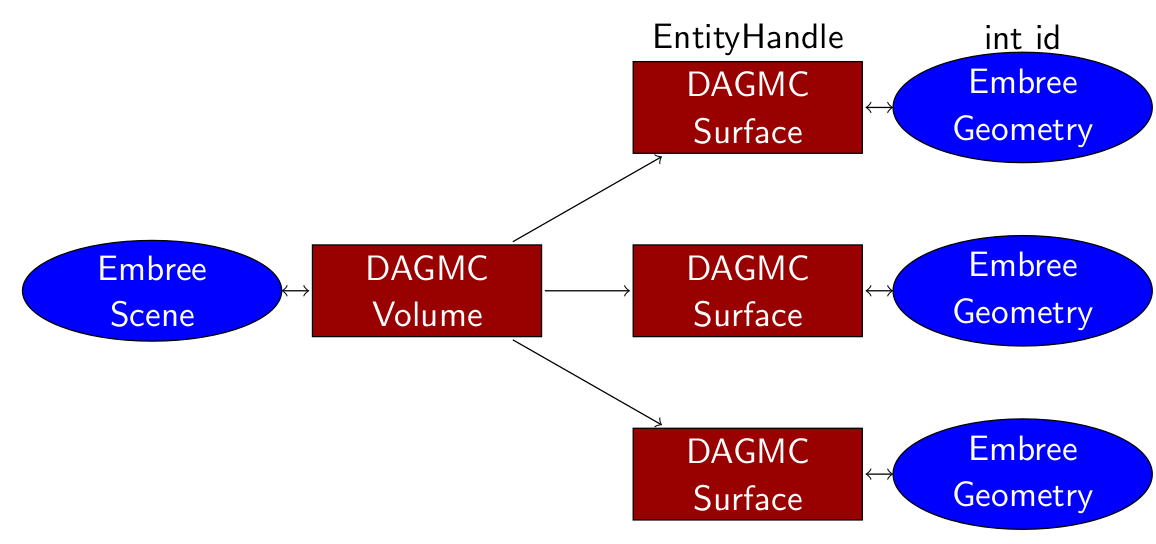
\includegraphics[scale=0.3]{emdag_mapping.png}
  \caption{Representation of MOAB tracking topological connections while mapped to Embree to perform ray queries.}
  \label{emdag_mapping}
\end{figure}

The representation of triangle normals are important to the DAGMC particle
tracking algorithm established by Smith et. al. in 2011 \cite{Smith_2011}. In
DAGMC, particles on or just outside the surface of a volume are handled by
ignoring the near-surface intersection upon being established in a new
volume. This is done to maintain tracking of particles based on their logical
position in the model rather than solely their numerical position which can
cause ambiguities regarding point containment and cause lost particles or
trapped particles between surfaces with infinite histories. Logical particle
tracking is implemented using the convention that triangle normals will always
point outward from the center of the volume they belong to. Triangles hit by the
ray are ignored if the normal of the triangle opposes the ray direction via a
dot product calculation to ensure only exiting ray intersections are
considered. While this has historically been handled inside of DAGMC, this is
accomplished in EmDAG via the use of Embree's filter functions. Filter functions
allow for a user-defined callback method which allows users to validate a ray
hit inside of Embree before returning a final result. Embree will return its
most recent intersection with the scene to the filter function (the hit
triangle's unnormalized vector included) and allow a method to either accept the
hit or instruct Embree to continute tracing the ray path based on the outcome of
the filter function. In MOAB, triangle normals are set in a global manner and
adjusted using stored information within MOAB based on what volume is being
queried at the moment. This is referred to as the surface's sense with respect
to that volume. Because we are forced to duplicate surfaces in Embree, the
triangle normals are pre-oriented based on this surface's sense for the scene it
is being created in upon initialization of the model within the Embree
instance. This saves steps in gathering this information upon traversal when the
triangle normal is needed to determine a particle's logical position within the
model. Though the connectivity of triangles is duplicated using this approach,
the overall memory footprint of EmDAG after duplicating the DAGMC geometry in
Embree is not much greater thanks to the single precision values for vertex
locations used in Embree which will be addressed in a later section of this
chapter.  By meeting DAGMC's requirements in the areas of topology, watertight
representation, and hit acceptance/rejection based on triangle normals, Embree
provides DagMC with all the information needed to perform geometric operations
required by the various Monte Carlo codes it supports, but in an agnostic manner
to the ray tracing kernel being used.

\subsubsection{EmDAG Performance Testing}%%Status:In Progress%%

Using the same DAGMC-based ray fire test program, the performance of DAGMC's ray
fire ability was compared to that of EmDAG's for three models. These models
include a simple sphere, a notched sphere, and a high aspect ratio cylinder. In
each of these tests, the models are tesselated with an increasingly smaller
faceting tolerance in a higher number of triangles and more complex nature of
the surface mesh in terms of BVH construction and traversal. The faceting
tolerance is defined as the maximum distance between the faceted curve or
surface and the geometric curve or surface which it resolves. 600k rays are then
fired from the center of the volume isotropically using the same random number
seed so that the same set of rays is fired in each ray tracing system.

\begin{figure}[H]
  \begin{center}
    \begin{tabular}{ccc}
      \includegraphics[scale=0.13]{sphere.eps} &
      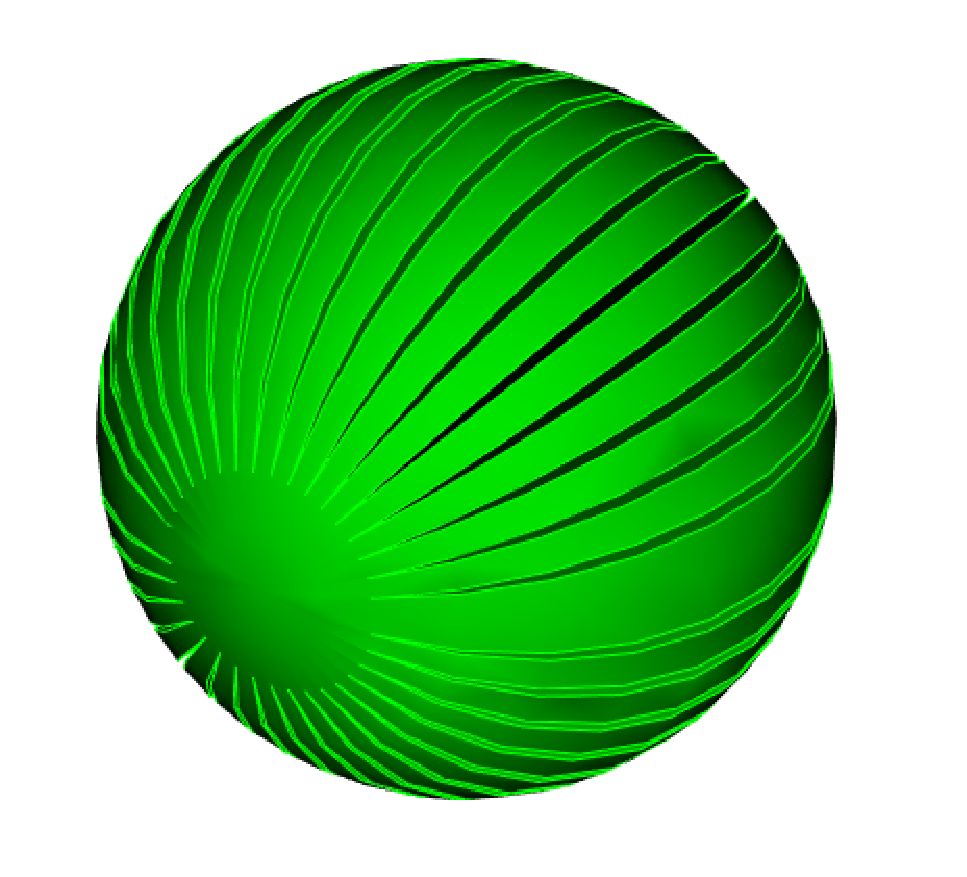
\includegraphics[scale=0.13]{ds.eps} &
      \includegraphics[scale=0.13]{larcyl.eps} \\
    \end{tabular}
    \caption{CAD representations of the sphere, slotted sphere, and high aspect
      ratio cylinder test models used for ray fire timings of DagMC and
      EmDagMC. (left to right) \label{models}}
  \end{center}
\end{figure} 

The sphere and slotted sphere models present speicalized challenges to the BVH
data structure as described in Section \ref{hv_study}. Due to memory contraints
of the system used for testing EmDAG's performance against DAGMC, the ITER
volume was removed and replaced with a high aspect ratio cylinder. The faceting
of the cylinder contains many long, thin triangles running along the barrel of
the cylinder. In similar fashion to the spherical model, the number of these
triangles will increase with decreasing faceting tolerance resulting in an
increasing triangle density as well. The low aspect ratio nature of these
triangles can cause difficulty in the calculations of tightly fitting OBBs
within MOAB's BVH builder. This test model is used to the ray tracing systems
robustness of the BVH generation algorithms to objects with surface meshes of
this nature.

The standard DAGMC ray fire test program (included in appendix A) was used to
evaluate both ray fire systems. The test program itself is agnostic to the
underlying ray tracing kernel used by DAGMC and two versions of the program were
compiled. One in which DAGMC uses MOAB's ray tracer and another in which MOAB's
ray tracing system is subverted by Embree, a.k.a. EmDAG. The two sets of timing
results can be found in Figure \ref{emdag_timing_compare}.

\begin{figure}[H]
  \vspace{-3cm}
  \centering
%  \includegraphics[scale=0.33]{Eig_fix_rf.ps}
%  \includegraphics[scale=0.33]{embree_rf.ps}
  \caption{A comparison of average ray fire times between DAGMC using MOAB's ray
    tracing and Embree. Please note the difference in time scale.}
  \label{emdag_timing_compare}
\end{figure}

Both MOAB and EmDAG scale relatively well for the HAR cylinder model with
decreasing faceting tolerance. This indicates that both systems are capable of
building bounding volumes well for a model with long, skinny triangles. The
scaling of the spherical case with increasing triangles is slightly worse than
the HAR cylinder most likely because the BVH tree is unavoidably going to
becomce gradually deeper as more and more triangles exist in the model. Finally,
the slotted sphere contains many high valence regions and as expected it scales
the worst with decreasing faceting tolerance as the valence of these regions
increases. It is very apparent that there is nearly an order of magnitude
difference in the ray fire timings MOAB and Embree. Due to the very similar
scaling of each test model, it can be stated that the majority of the
descrepancy in the ray fire timings between the two systems occurs in the
traversal methods employed by both systems and isn't likely due to a significant
difference in the structure of the BVH being built by either system. Changes in
the way the BVH is built typically accounts for anywhere from 30-40\% difference
in ray fire timings whereas the descrepancy seen here between MOAB and Embree is
on average \textbf{an order of magnitude better} when using Embree. In large
part, this has to do with Embree's freedom of design without the restriction of
a ray tracing implementation inside the context of another application. MOAB's
flexibility in core design allows for the robust implementation of an oriented
bounding box tree within this context, but comes with the overhead of database
calls to retreieve stored information which can be undesirable for a
high-performance system and doesn't allow MAOB to take advantage of some
implementation optimizations that Embree does. The vectorization of Embree's
traversal through its BVH contributes greatly to its speed. This can be also
considered a part of the design freedom allowed when designing an independent
ray tracing system that cannot not be afforded using only MOAB's database
interface. However, a property unique to MOAB may allow for an implementation
such as this as will be discussed near the end of this work.

\subsection{EmDAG Transport Tests}
\label{subsec:emdag_transport}

As an extension of these pure ray fire tests, the effect of an improved ray
tracing system on particle transport was studied as well. These tests begin with
several simple models and end with the application of EmDAG to one of the models
used for DAGMC performance benchmarking in Chapter \ref{perf_benchmark}, FNG.

The first transport models to be tested were a single cube and single sphere
filled with a dense hydrogen material for high collisionality in the problem
resulting in a large number of ray queries in the transport run. Each of these
models' principal dimension is 10 cm. The source for these models is a 5 MeV
neutron isotropic point source at the center of the volume. One million
particles were simulated in each test. All of the test models were preproccessed
using a faceting tolerance of $10^{-4}$cm. Moving upward in complexity, another
set of tests were run using a set of nested cubes and nested spheres. Each of
the nested volume models contained three cells: the inner volume, a shell
volume, and the graveyard volume. The purpose of these tests was to ensure that
particles could in fact be tracked through multiple volumes robustly. The nested
cubes model contains an extra volume which consists of the original single cube
subtracted from a cube 1cm larger in each dimension. The nested sphere model
contains an extra volume consisting of the original sphere from the single
volume model subtracted from a sphere 1cm larger in radius. As the purpose of
these tests was to test EmDAG's particle tracking between non-zero importance
cells, the dimensions of the offset between the nested volumes is largely
irrelevant so long as particles are in fact reaching all of the cells.

\begin{table}[H]
  \small
  \begin{center}

      \label{timings}
    \begin{tabular}{lccc}

      \toprule
      Test Model & MCNP & DagMCNP & EmDagMCNP \\
      %%\hline
      & \multicolumn{3}{c}{\textbf{time (min)/ ratio to MCNP}} \\
      \hline
      Sphere & 2.93 / 1.00 & 25.13 / 8.58  & 4.73 / 1.61  \\
      Cube & 5.03 / 1.00 & 10.56 / 2.10 & 5.80 / 1.153 \\
      Nested Spheres & 4.35 / 1.00  & 50.82 / 11.68  & 7.94 / 1.83 \\
      Nested Cubes & 4.73 / 1.00 & 9.26 / 1.96 & 4.35 / 0.92 \\
      %%\hline
      &  \multicolumn{3}{c}{\textbf{histories/min}} \\
      \hline
      Sphere & 3.4104E+05  & 3.9944E+04  & 2.1810E+05   \\
      Cube & 1.9879E+05 & 9.4738E+04 & 1.7260E+05 \\
      Nested Spheres & 2.2991E+05 & 1.9877E+04 & 1.3947E+05 \\
      Nested Cubes & 2.1170E+05 & 1.0806E+05 & 2.3026E+05 \\
      \bottomrule
      
    \end{tabular}
  \end{center}
  \caption{Runtime comparison native MCNP, DAG-MCNP, and EmDAG-MCNP over four
    transport test problems.}
  
\end{table}

The native MCNP runs were generally the fastest among the test problems with the
exception of the nested cubes case in which EmDAG-MCNP marginally outperformed
the native code by ~8\%. This is likely due to the fact that very few triangles
are needed to exactly represent the surfaces of cubic volumes. This creates a
very simple problem in the area of BVH building and results in a shallow
tree. The fact that these volumes have multiple surfaces is also of importance
here. MCNP searches linearly through a given cell's (volume's) surfaces to
determine the intersection of a particle with the nearest surface whereas both
DAG-MCNP and EmDAG-MCNP perform this search spatially. In the nested cubes
model, it is likely that the number of surfaces relative to the number of
triangles in their representation is high enough to allow EmDAG-MCNP to overtake
MCNP's CSG calculations. This is a good demonstration of how CSG implementations
suffer from the lack of a spatial search component when creating volumes from
boolean combination of surfaces as mentioned in Section \ref{implicit_surfaces}.

\begin{table}[H]
  \small
  \begin{center}
    \begin{tabular}{lccc}
      \toprule
      Value & MCNP & DagMCNP & EmDagMCNP \\
      \toprule
      %%Hist/min & 2.2991E+05 & 1.9877E+04 & 1.3947E+05 \\
      %%\hline
      \multicolumn{4}{l}{\textbf{Cell 1 Tallies}} \\
      \hline
      Flux  & 5.25725E-03 & 5.25734E-03 & 5.25734E-03 \\
      Energy  & 3.17869E-03 &  3.17873E-03 &  3.17873E-03 \\
      \hline
      \multicolumn{4}{l}{\textbf{Cell 2 Tallies}} \\
      \hline
      Flux  & 1.91645E-04 & 1.91644E-04 & 1.91644E-04 \\
      Energy  & 5.22131E-05 & 5.22137E-05 & 5.22137E-05 \\
      \hline
      \multicolumn{4}{l}{\textbf{Cell 3 Tallies}} \\
      \hline
      Flux  & 1.18371E-05 & 1.18376E-05 & 1.18410E-05 \\
      Energy  & 4.96282E-06 & 4.96285E-06 & 4.96285E-06 \\
      \bottomrule
                        
    \end{tabular}
    \caption{Nested Spheres Tally Results. Flux tally units are
      $cm^{-2}$. Energy tally units are MeV/g. Note: result comparisons of other
      test cases can be found in Appendix B.}
    \label{nestedspheres}
  \end{center}
%%\vspace{-0.2cm}
\end{table}


The results of the single-volume test cases for native MCNP differ slightly from
the agreeing tally results from the DAGMC-based systems. This is not surprising
as DAGMC is known to report slightly different results from native MCNP. As
result comparisons of DAGMC to native codes are not the concern of this study,
only a comparison of the values returned by EmDAG in comparison to DAGMC is
considered. Differences in the tally results between DAG-MCNP and EmDAG-MCNP are
present only in the nested spheres transport model. There is a small difference
in the flux tally for cell 3 as can be seen in Table \ref{nestedspheres}. By
examining the number of particle tracks in each cell, it can be determined that
this discrepancy is caused by a single particle ending in EmDAG-MCNP near a
surface of cell 2 while in DAG-MCNP the particle crosses into cell 3 before
abruptly terminating though it still contributing slightly to the tally in cell
3. It is believed that this difference in tally result is the result of a
systematic difference between Embree and MOAB's ray fire conventionality rather
than Embree's a result of the double to single floating point conversion of the
model that occurs when using EmDAG though this difference in precision is
suspected to be problematic in other ways as was discovered in transport on the
FNG model.

Finally, a full-scale test of EmDAG was conducted on the FNG model using the
same volumetric source as in the performance benchmarking tests described
earlier. Initially this model failed quickly due to lost particles. This was
surprising as the model is expected to have the same watertight fidelity that it
does when using DAGMC. In order to allow the run to complete, the number of
allowed lost particles was increased to the number of the sources particles
being run (1e8). The justification for this allowance being that if the lost
particle rate is small enough, overall performace and results of the run would
still provide a viable comparison of the two systems. In the end, the model lost
255 particles in 100 million histories. While this is concerning in terms of
robustness, the lost particle rate per history wasn't considered high enough
greatly impact the results from a performance comparison standpoint. A timing
comparison of the FNG run using EmDAG-MCNP to the native MCNP model as well as
DAG-MCNP is found in Table \ref{fngemdag}.

\begin{table}[H]
  \small
  \begin{center}
        \begin{tabular}{|c|c|c|c|c|}
      \hline
      \textbf{Implementation} & \textbf{ctme (min)} & \textbf{wall time (min)} & \textbf{ratio} & \textbf{lost} \\
      \hline
      MCNP5 & 209.92 & 205.99 &  1.00 & 0 \\
      \hline
      DAG-MCNP5 & 1023.04 & 1023.05 & 4.99 & 0  \\
      \hline
      DAG-MCNP5 (lt) & 974.99 & 974.75 & 4.73 & 0  \\
      \hline      
      EmDAG-MCNP5 & 303.49 & 303.63 & 1.44 & 255  \\
      \hline
      EmDAG-MCNP5 (lt) & 257.49 & 257.60  & 1.25 & 247 \\
      \hline
    \end{tabular} 
    \caption{A comparison of transport on the FNG model using a 14.1 MeV
      volumetric source over 100M histories for native MCNP, DAG-MCNP, and
      EmDAG-MCNP.}
    \label{fngemdag}
  \end{center}
\end{table}


\begin{figure}
  \centering
  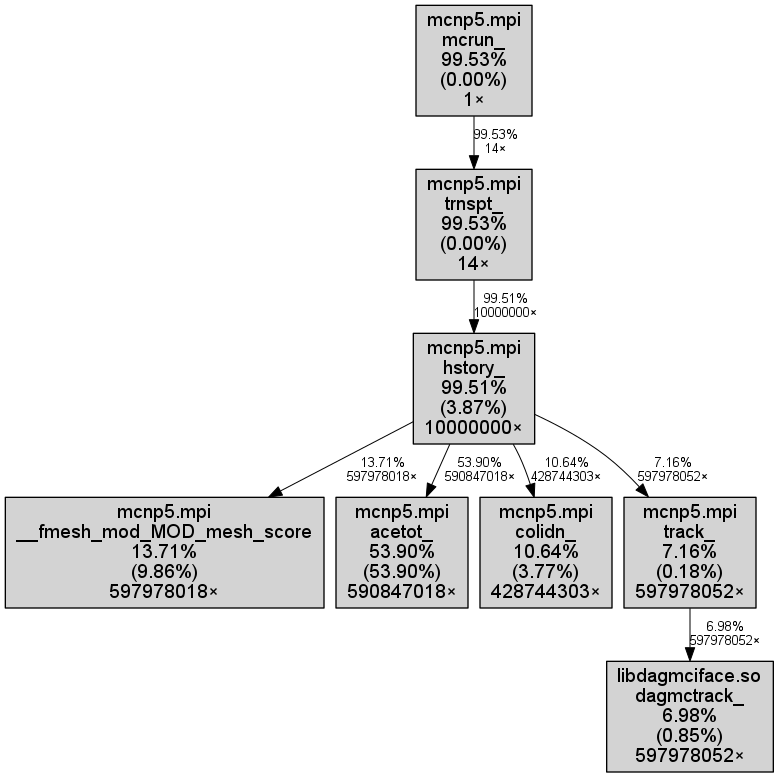
\includegraphics[scale=0.45]{emdag_fng_cg_fine6.png}
  \caption{Callgraph of the EmDAG run on the FNG model for 1E7
    histories. (Processes taking $>=$6\% of the runtime are filtered in order to
    siplify the callgraph.}
  \label{emdag-fng-coarse}  
\end{figure}

While the performance of EmDAG greatly surpases that of DAGMC, it does not come
as close to the performance of native MCNP as it did in the more simple
transport test models. Upon visually inspecting the faceted FNG model, it was
seen to contain many high valence regions. As an artifact of the variance
reduction used in the intended analysis of this model, many planes were inserted
in the model in order to break up large cells with highly varying particle
intensities. Where these planes intersect the cylindrical volumes of the model,
many high valence regions result as can be seen in Figure
\ref{fng-faceted-models}. As a result it became a curiousity as to whether or
not the high valence regions were being handled better by EmDAG than they were
by DAGMC. In order to test this, the same programs used to do the high valence
vertex study were built using EmDAG and the parameter study of the relative high
valence area and valency was performed. The results in Figure \ref{emdaghvstudy}
show that EmDAG also struggles with these high valence regions. In the worst
scenario there is a degradation by two orders of magnitude compared to the best
case scenario which is similar to what seen in the unmodified MOAB ray
tracer. Additionally, it shows degraded performance in the same way that DAGMC
was initally expected to falter - with increasing high valence area and
valency. This is likely due to the nature of the heuristics used by Embree to
construct its acceleration datastuctures.  Unlike MOAB, however, the BVH
building parameters are not as openly available via Embree's interface.There is,
however, an option to reduce the size of the high valence regions in the mode
within the faceting algorithm by definig a length tolerance.

\begin{figure}[H]
  \small
  \begin{center}
    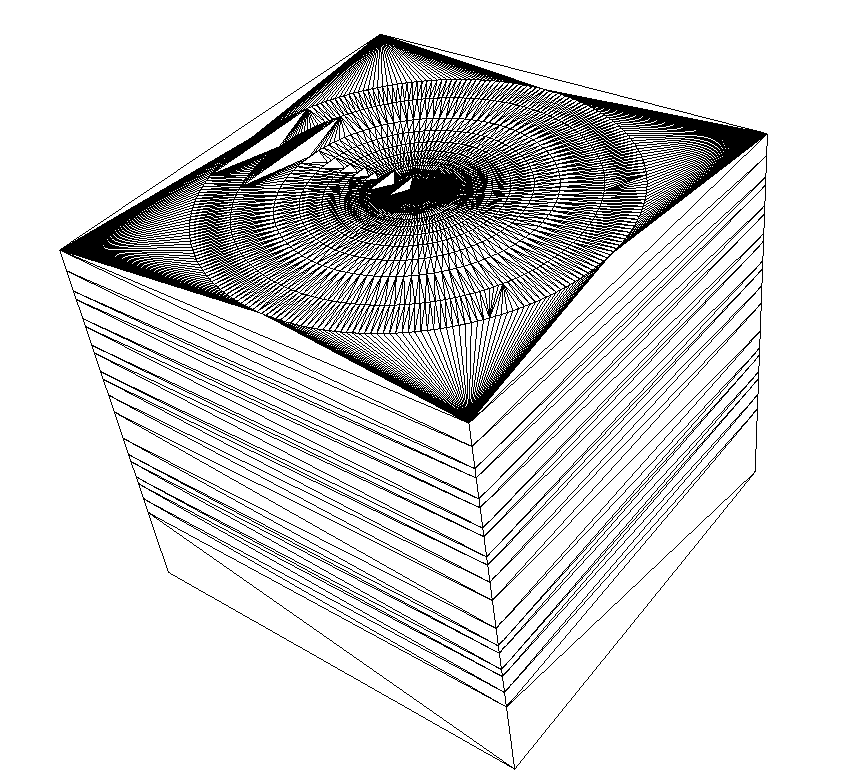
\includegraphics[scale=0.3, trim = 200 0 100 0]{fng_facet_tol.png}
    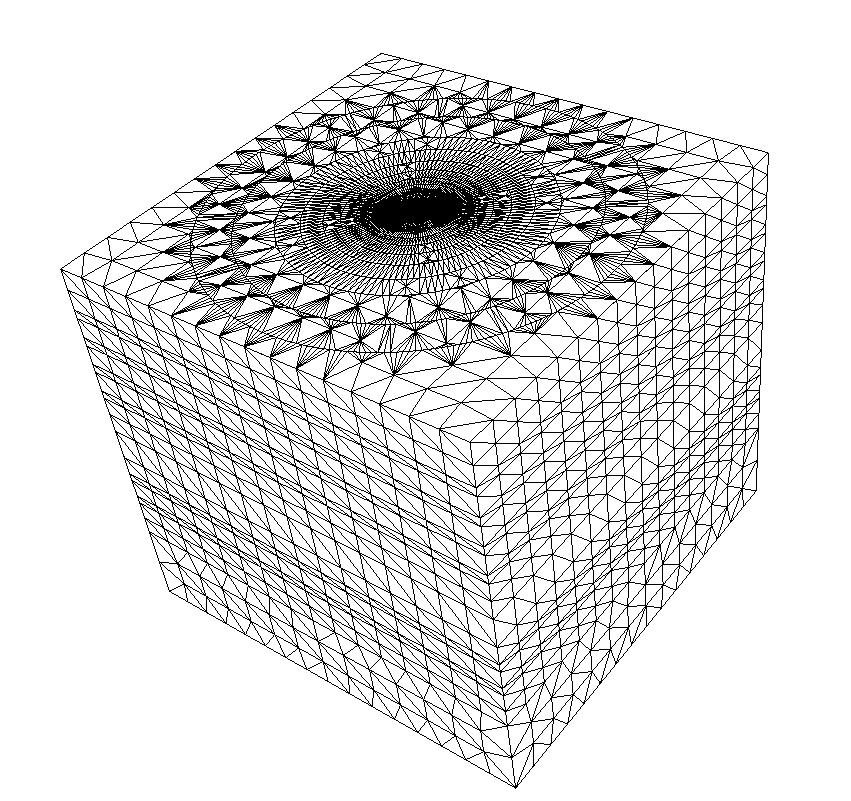
\includegraphics[scale=0.25]{fng_len_tol.png}
    \caption{The FNG faceted model without (left) and with (right) the length
      tolerance applied.}
    \label{fng-faceted-models}
  \end{center}
\end{figure}

The length tolerance is a maximum length for any facet edge returned by the CAD
engine's faceting algorithm. Providing this value to the preprocessing tool
comes at the cost of many more triangles than when supplying only a faceting
tolerance. The difference in facet structure between these models can be seen in
Figure \ref{fng-faceted-models}.

By generating a faceted model using the combination of the length and faceting
tolerances it was hoped that there would be a marked increase in performance
using the EmDAG system and the performance did indeed improve by ~15\%. Due to
the increased number of overall triangles on these planar surfaces, there may be
competing forces at play. As the length tolerance is reduced, the high valence
areas will also be reduced, but the overall number of triangles will increase -
resulting in inherently deeper BVH and longer traversals. Conversely, as the
length tolerance is increased, the number of high valence region areas are
increase, but the number of redundant triangles is reduced improving the average
BVH traversal time enough compensate for a few more rays entering high valence
regions. This observation leads to the idea that length tolerance of the FNG
model could then be optimized. This optimization study, while interesting, will
vary model to model and the results will be complex in nature, depending on the
underlying geometry and geometry adjacent to those regions, etc. In light of the
high valence study results showing that BVH building parameters can be altered
to improve performance and accomodate these high valence regions, it seems that
a better solution is to follow that path over alteration of the mesh globally in
the model. 

\subsubsection{Limitations of the EmDAG system}%%Status:In Progress%%

While the implementation of Embree in DAGMC showed a vast improvement in
performance relative to DAGMC's current implementation, several problems were
encountered during the process. This is not surprising when repurposing a ray
tracing kernal for an unintended application.

One of these problems is the presence of lost particles in a watertight
model. The FNG model EmDAG was tested on is a fully sealed model via the
make\_watertight algorithm. A fully sealed model is one in which every volume is
topologically sealed such that there are no gaps between surfaces or adjacent
volumes. As a result, DAGMC is able to robustly track particles through such a
model with no lost particles. While the lost particle rate for the EmDAG FNG
test relatively low, they in theory should not occur at all as was shown by the
DAGMC runs. After a considerable amount of investigation as to the nature of
these lost particles, their cause was determined to be systematic problem not
encountered in the nested volume cases due to the simple nature of their
geometric topology.

In the DAGMC workflow, a required step for a watertight model is to imprint and
merge the surfaces within the CAD system before faceting the model. Imprinting
is the process by which Trelis, the CAD software used to generate DAGMC models,
makes surfaces and curves that are coincident in space be fully coincident. This
process is accomplished by splitting entities into their coincident and
non-coincident parts. The merging process then topologically combines these
coincident parts into single entities such that the single entities are
topologically adjacent to all entities bounding the original set of entities
that were merged into one. The result of these steps is non-manifold model with
surfaces shared between neighboring volumes \cite{Smith_2011}.

This imprinting and merging of surfaces allows only one representation of each
topological entity to be created upon faceting the model. By using the faceted
curves of the model as a reference for where surfaces meet in space, the
triangles of a surface are then made to meet at those curves in a topologically
watertight manner via the \textit{make\_watertight} algorithm. Topologically
watertight in reference to triangle facets refers to shared connectivity between
surfaces which is distinctly different than watertight by proximity. This
topological watertightness of mesh refers to the fact that triangle surfaces
meshes have connectivity at their interface which share vertex handles inside of
the MOAB database. These vertex handles will then point to the \textbf{exact
  same floating point representation} of the vertices no matter which of the
surfaces is being queried. In this way particles are not lost through gaps in
surfaces and firing a ray from the logcal position inside a volume should always
result in a triangle intersection. This is not the case however when using
EmDAG. Particles were somehow being lost in the transport process.

\begin{figure}[H]
  \centering
  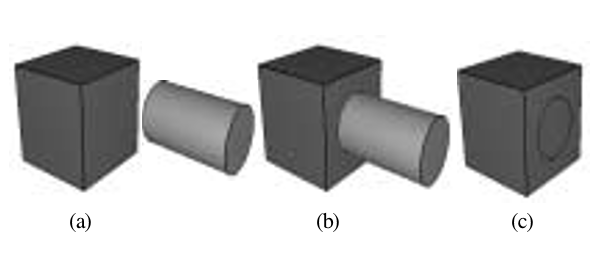
\includegraphics[scale=0.5]{imprint_ex.png}
  \caption{Example of two adjacent volumes being imprinted and merged. a) Two
    volumes, a cube and cylinder are created. b) The cylinder end face is moved
    such that it is coincident with one of the faces of the cube. c) The imprint
    operation is performed and the cylinder curve is imprinted onto the cube
    (cylinder was removed for visibility of imprinted curve). Adapted from
    \cite{White_2002}.}
  \label{imprint_ex}
\end{figure}

Some detailed debugging of this problem revealed that this occurs in a
systematic fashion within the FNG model at intersections of 3 or more
volumes. The secnario is that a particle moves into the intersection between two
surfaces. When this occurs, an intersection with either surface connected to
that interface is a valid hit so long as the surface is part of the volume the
particle is current positioned within. The particle will then logically move
into the volume on the other side of the hit surface. EmDAG handles most of
these cases well but for the case in which a particle will have a zero track
length inside one of the volumes. A zero track length in this case meaning that
the particles trajectory is such that it will only glance a volume without
having any appreciable track length inside of it. In this case, the EmDAG system
may be unable to find a hit whereas DAGMC's tracking is robust enough to find
the triangle intersection on this volume and move on.

\begin{figure}[h!]
  \begin{centering}
    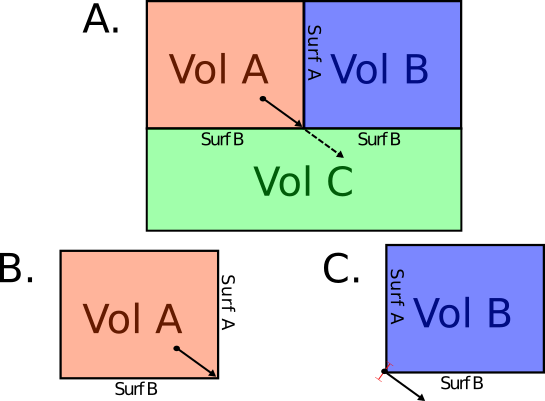
\includegraphics[scale=0.7]{emdag_lost.png}
    \caption{\textbf{A)} The initial scenario of the lost particle. The
      particle's trajectory is such that it intersects with the boundary between
      surfaces A and B. The correct continuation of the particle into volume C
      is depicted as a dashed line. \textbf{B)} An intersection with surface A
      is found though either surface A or B are equally valid. The particles
      position is then updated to its intersection with the boundary of surfaces
      A and B. The particle then logically moves into volume B. \textbf{C)} Upon
      establishment of the particle in volume B the Monte Carlo code requests
      the distance to next surface intersection. The particles position and
      direction are converted from double to single precision. The small change
      in the particle's position places it outside of volume B and the
      trajectory is such that an intersection is not found. At this point the
      particle is considered lost.}
    \label{emdag-lost-particles}
  \end{centering}
  \end{figure}

By isolating this particle's history and producing the particle history with
locations precise enough to detect the descrepancies between EmDAG and DAGMC, it
was found that the position of the particle in EmDAG was numerically too far
outside of a volume to produce the correct triangle hit in either EmDAG or
DAGMC's ray fire systems. The cause of this descrepancy is believed to have to
do with the necessary conversion between double and sinble floating point
precision in the EmDAG system.

As mentioned before, EmDAG uses single floating point representation in its ray
tracing kernel while DAGMC uses a double precision representation of the
geometry and particle information as does MCNP. In order to accomodate Embree's
representation, properties of the particle location and direction are converted
to single precision for ray tracing queries in Embree and back to double
precision when in DAGMC. When changing the floating point representation,
rounding rules based on the computing environment are used to determine the new
representation according to IEEE standards for conversion between precision
levels \cite{IEEE_STD_2008}. These changes in the particle's location and
direction are small, but in the scenario described above it seems that the
particle location and/or direction are altered enough throughout the course of
its history to cause a failed ray intersection - resulting in a lost particle.

In Brandon Smith's thesis, ``Robust Particle Tracking and Advanced Geometry for
Monte Carlo Radiation Transport'' \cite{Smith_2011} there is a detailed
description of the different pathologies encountered in tracking particles
through a surface mesh representation of a geometric model. Briefly mentioned in
this chapter is the possibility of a lost particle due to numerical error in the
particle's position perpindicular to the particle's trajectory. Lost particles
caused by this pathology are not covered however as the double floating point
representation does not allow the particle position to change enough for this
case to occur in practice. In EmDAG, however, this particular pathology is now
vulnerable due to the constant conversion from single to double precision values
between DAGMC and Embree. In order to avoid this problem moving forward, any
improvements to DAGMC's ray tracing kernel for particle tracking will need to
maintain use of double precision representations for mesh elements for robust
coupling of numerical and logical particle positions and directions.
